Den grafiske brugergrænseflade er først og fremmest lavet ud fra et design som Katrines kælder
har ønsket. Dette design er baseret på det eksisterende kasseaparats tastatur og mærkater, således
at overgangen fra at skulle bruge det gamle kasseaparat til det nye ville mindskes.
Hertil er der blevet tegnet et skitse som kuhnne bruges til at lave et mock-up af den kommende GUI. På figur \ref{fig:GUTskitse} kan skitsen af GUI'en ses.\newline

\begin{figure}[H]
\centering
	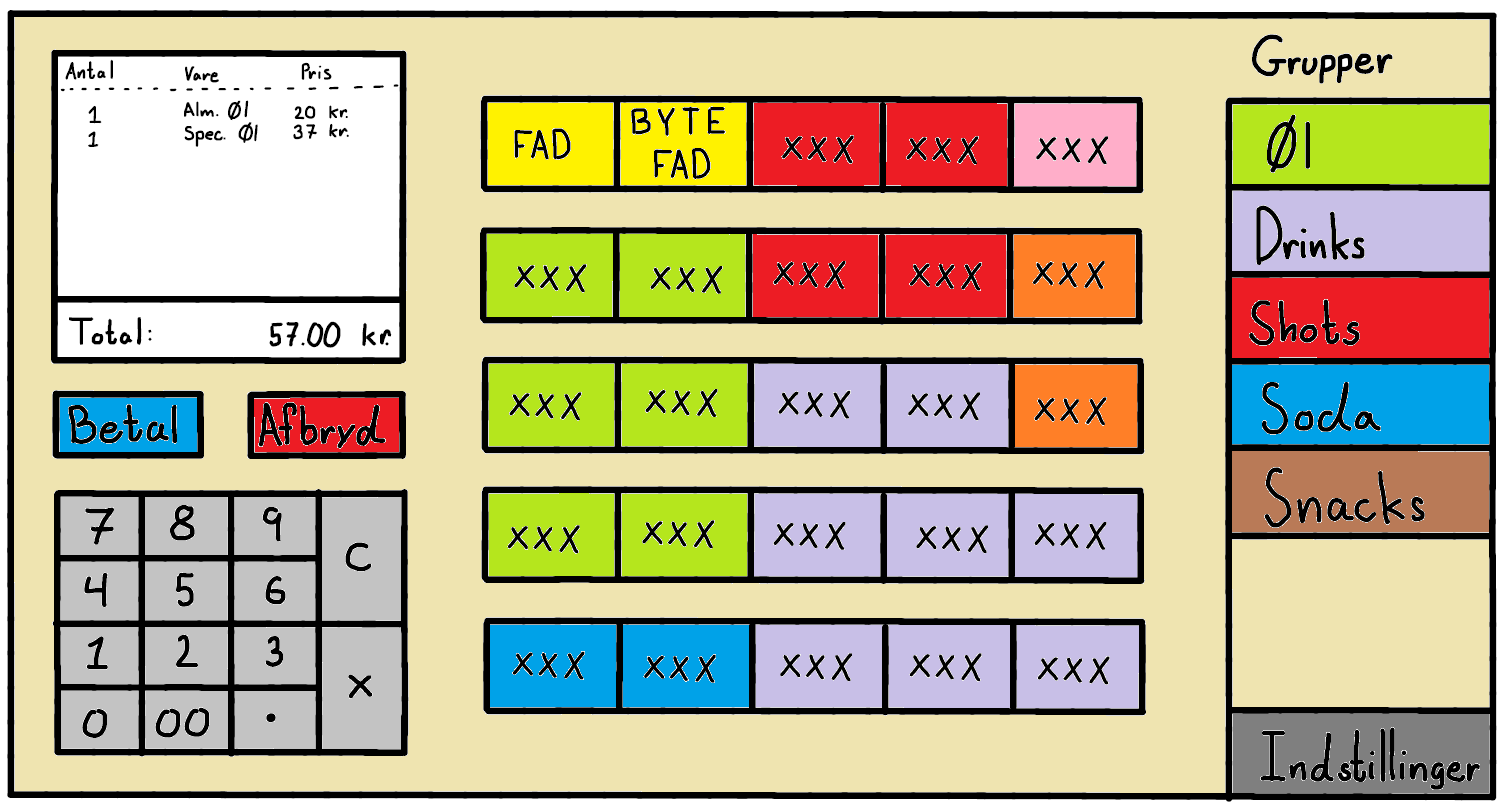
\includegraphics[scale=0.5]{Kravspecifikation/Interface/Interface1F.png}
	\caption{Skitse af GUI}
	\label{fig:GUTskitse}
\end{figure}

\subsubsection{Mock-up}
Det første mock-up blev lavet som en ren illustrativ GUI uden nogen form for funktionalitet. Hertil
blev den lavet uden fornemmelse for hvad der var smart men kun med tankerne om hvordan den
kunne ligne det gamle kasseaparats tastatur. På figur \ref{fig:GUIMock} kan udkastet til GUI'en ses.
\begin{figure}[H]
\centering
	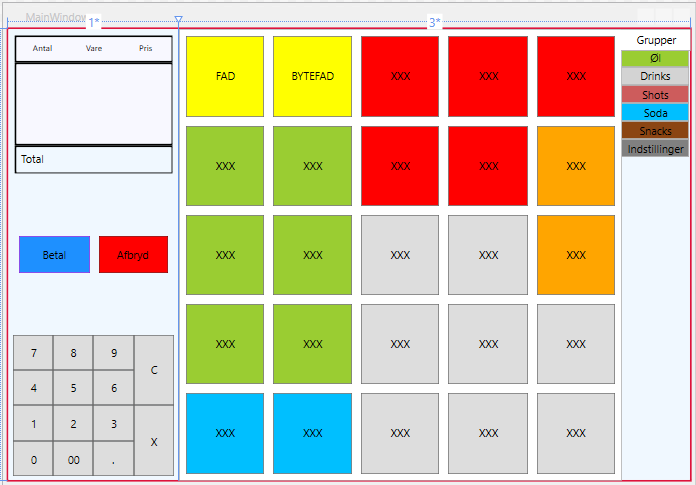
\includegraphics[scale=0.8]{Rapport/GUIMockUp.PNG}
	\caption{Mock up af GUI}
	\label{fig:GUIMock}
\end{figure}
\subsubsection{MVVM}
Da det første mock-up var lavet gik der et sprint hvor der intet GUI blev lavet. Sprintet var mere fokuseret på business logik. Herefter blev der taget fat i GUI’en igen hvor selv hovedvinduet blev delt i tre
UserContents. Dette var smart da det blev aftalt at GUI’en skulle laves efter MVVM princippet
og her kunne de tre usercontents så repræsentere et view hver. Til hver af disse views skulle der så
laves en tilhørende viewModel som kunne hente data fra businesslogikken således at Viewet ikke
skulle tænke på dette selv. Den tilhørende viewmodel skulle nemlig modellere viewet alt efter hvad
der skete i businesslogikken. Dette blev gjort med Bindings fra View til Viewmodel, Og Events fra
businesslogik til Viewmodel.
Selve udseendet af GUI’en blev præget meget af Resources der skulle gøre det hele mere ensartet.
Hertil er der blevet dataTemplates, styles og bindings mm.
Den færdige GUI kom til i sin enkelthed at ligne det mock-up der blev lavet, men der kom meget
mere fokus på hvilke controls der var smarte, og hvilke der ikke var smarte og så fik den en fin
afpusning der gjorde den pænere at se på. På figur \ref{fig:GUIFinal} kan der ses hvor dan GUI'ens endelige udsende blev.

\begin{figure}[H]
\centering
	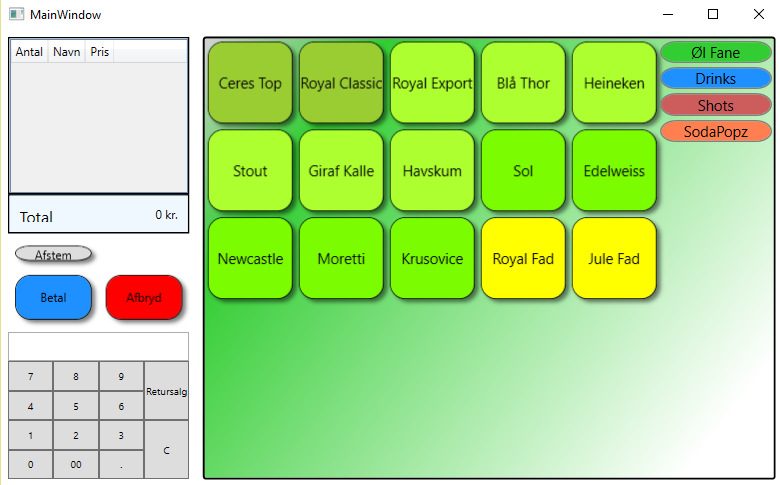
\includegraphics[scale=0.8]{Rapport/GUIFinal.PNG}
	\caption{Endelig udgave af GUI}
	\label{fig:GUIFinal}
\end{figure}

\subsubsection{Dynamik}
Selvom det ikke er til at se i figur \ref{fig:GUIFinal} så er alle produktknapperne dynamisk oprettede. 
En vigtig del af GUI designet var at det skulle være nemt at tilføje/fjerne de produkter der blev solgt.
Dette har vi opnået ved at lade ViewModel stå for at oprette knapperne, dette er gjort ved at have \texttt{ObservableCollections} som der er lavet databind på i \texttt{XAML} koden.
De \texttt{ObservableCollections} gør også at \texttt{XAML} koden kun beskriver hvordan udsendet skal være, da alle knapperne ligger i den \texttt{ObservableCollection}
